\section{State of Research} \label{sec:state_of_research}

Before presenting the methodology of the study in Section \ref{sec:methodology}, this section provides an overview of the state of research relevant to this thesis. It is structured into three main sections: Section \ref{ssec:xai} presents research into \ac{XAI}, Section \ref{ssec:cognitive_psychology} discusses relevant theories and findings from cognitive psychology, and Section \ref{ssec:cognition_ai_users} presents research into how users cognitively process \ac{AI} output in decision support systems and \acp{LLM}.

\subsection{Explainable AI} \label{ssec:xai}

This Section provides an overview of \ac{XAI} by first defining key terminology in Section \ref{sssec:terminology}, which clarifies the distinctions between interpretability, explainability, and transparency as well as the differences between generative and discriminative \ac{AI}. It then discusses the state of research for explainability methods in Section \ref{sssec:explainability_methods}, highlighting both traditional approaches and recent advancements in the field.

\subsubsection{Terminology} \label{sssec:terminology}

While in the field of \ac{XAI} the terms \textit{interpretability} and \textit{explainability} are often used interchangeably, in cognitive psychology they have distinct meanings. \textit{Interpretability} is a broad concept that encompasses various ways to “provide the meaning in understandable terms to a human” \parencite{Arrieta2020}. \textit{Explainability} is one of these modes, that uses an explanation to convey this meaning \parencite{Lipton2016}. \textit{Transparency} is another mode of \textit{interpretability} that conveys meaning by making the inner workings of a model visible to a human \parencite{Arrieta2020}. The limiting factor for \textit{transparency} is the human's ability to understand the inner workings of a model. \textit{Explainability} on the other hand can be applied to any model, regardless of its complexity, by using post-hoc explainability methods \parencite{Arrieta2020}.

The most important distinction for this thesis is between generative and discriminative models. Conceptually generative and discriminative \ac{AI} both use machine learning to learn patterns from data. They are however fundamentally different in their application. Discriminative models learn the decision boundary between two or more classes and are used for classifying data points into these existing classes. Common use cases include anomaly detection \parencite{Edozie2025, Hilal2022}, image classification \parencite{Lu2007}, and sentiment analysis \parencite{Wankhade2022}. Generative models on the other hand learn the underlying distribution of a dataset and can be used to generate new data points that are similar to the training data. Generative models are frequently used for text generation \parencite{Brown2020} or image synthesis \parencite{Rombach2021}.

In the context of \ac{XAI} generative and discriminative models differ in one key aspect: the type and size of output they produce. In an information theoretical sense, discriminative models produce a small amount of information, like a class label that can be expressed in possibly a few dozen bits in extreme cases \parencite{Schneider2024}. Furthermore, the output is often previously known in the form of existing classes. Generative models on the other hand produce a large amount of information, like a paragraph of text or an image, that can be expressed in the order of megabits \parencite{Schneider2024}. Furthermore, the output is often novel and not previously known. This difference in output has implications for explainability methods and how users interact with and perceive these models. Discriminative models can be designed to be inherently interpretable by using simple models like decision trees or linear regression \parencite{Rudin2019}. Alternatively post-hoc explainability methods can be used to explain complex models like deep neural networks \parencite{Ribeiro2016, Lundberg2017}. Generative models on the other hand are often complex and not interpretable by design, which limits the applicability of inherently interpretable models.

\subsubsection{Explainability Methods} \label{sssec:explainability_methods}

Much research in \ac{XAI} has focused on developing explainability methods for discriminative models. These methods can be broadly categorized into two groups: transparency-based methods and post-hoc explainability methods \parencite{Arrieta2020}. Transparency-based methods aim to make the inner workings of a model visible to a human. This can be achieved by using simple models like decision trees or linear regression that are inherently interpretable \parencite{Rudin2019}. Post-hoc explainability methods on the other hand aim to explain the output of a model without making its inner workings visible. This is achieved by highlighting important features in the input data (like LIME \parencite{Ribeiro2016}) or by approximating the model with a simpler interpretable model (like SHAP \parencite{Lundberg2017}). While these methods have proven to be effective in explaining models, both approaches are very technical and are difficult to understand for non-experts \parencite{Martens2025}.

Recently, new explainability approaches have been proposed that seek to remedy these shortcomings. Counterfactual explanations \parencite{Wachter2017} provide explanations by explaining why an alternative output was not chosen. For example in a loan application, a counterfactual explanation could state that if the applicant had a higher income, the loan would have been approved. Another approach are narrative explanations which use natural language to construct a short narrative around SHAP or counterfactual explanations \parencite{Martens2025}. While experts saw little benefit from narrative explanations, non-experts found them significantly more useful and easier to understand \parencite{Martens2025}.

A third approach involves \ac{CoT} explanations \parencite{Wei2022}, where \acp{LLM} generate intermediate reasoning steps that lead to the final output. These steps can enhance users' perception of transparency by allowing them to follow the model's reasoning process. Moreover, decomposing complex problems into smaller steps has been shown to improve the effectiveness of \acp{LLM} in problem-solving \parencite{Wei2022}. Notably, this technique can be applied to existing models without retraining, as demonstrated in this study. However, it is important to recognize that these intermediate steps are generated by the model itself and may be unfaithful or incorrect \parencite{Turpin2023, Schneider2024}. In a related line of research, \textcite{Lindsey2025} demonstrated that it is possible to identify and visualize specific neurons representing concepts, and to observe activation patterns that resemble a thought process.


\subsection{Cognitive Psychology} \label{ssec:cognitive_psychology}

This Section provides an overview of relevant theories and findings from cognitive psychology. To establish a framework for understanding human cognition, Section \ref{sssec:dual_process} discusses dual process theory. Sections \ref{sssec:heuristics} and \ref{sssec:metacognition} discuss heuristics and metacognition to further elaborate on cognitive processes relevant to this thesis. Finally, Section \ref{sssec:cognitive_offloading} discusses cognitive offloading as this behaviour and its drivers are particularly relevant to human-AI interaction.

\subsubsection{Dual Process Theory} \label{sssec:dual_process}

Dual process theory refers to a group of theories in cognitive psychology that proposes humans have two distinct types of cognitive processing: Type 1 and Type 2 \parencite{Evans2013}. Type 1 processing is intuitive, autonomous processing and often referred to as “System 1” \parencite{Kahneman2011}. Type 2 processing (also “System 2”) on the other hand is deliberate, controlled processing that requires cognitive effort \parencite{Evans2013}. It is often associated with higher-order cognitive functions like reasoning, problem-solving, and decision-making \parencite{Kahneman2011}. Different theories propose different characteristics for both types of processing, but they agree on several core characteristics as summarized in Table \ref{tab:dual_process_characteristics}. The first two rows contain characteristics that are widely agreed upon, while the remaining rows contain characteristics, that find support in some theories, but are not as universally accepted \parencite{Evans2013}.

\begin{ctable}
    \begin{tabular}{l|l}
        \textbf{Type 1} & \textbf{Type 2} \\
        \hline
        Autonomous & Deliberate \\
        Intuitive & Controlled \\
        \hline
        Fast & Slow \\
        Parallel & Serial \\
        Non-conscious & Conscious \\
        Biased responses & Normative responses \\
        Contextualized & Abstract \\
    \end{tabular}
    \caption[Type 1 and Type 2 Characteristics]{Common characteristics of Type 1 and Type 2 processing in dual process theories \parencite{Evans2013}}
    \label{tab:dual_process_characteristics}
\end{ctable}

Different theories propose different relationships between Type 1 and Type 2 processing. Some theories propose a competitive relationship, where both types of processing work in parallel and resolve conflicts if they occur. However, this conflicts with the fact that the two systems are associated with different speeds. If Type 1 processing is faster, conflict resolution would always have to wait for Type 2 processing to finish. Alternatively, a wide range of theories proposes a default-interventionist relationship, where Type 1 processing is the default mode of processing and Type 2 processing only intervenes when necessary \parencite{Evans2013}. There is evidence for both relationships, even attempts to reconcile both relationships into a single theory, but the exact relationship remains an open question \parencite{Evans2013, Djulbegovic2012}. Recent research in the context of \ac{XAI} has interpreted results assuming the default-interventionist relationship is the more accurate one \parencite{Jussupow2021, Shin2021}.

\subsubsection{Heuristics} \label{sssec:heuristics}

Heuristics are methods for problem-solving that use practical and efficient approaches to produce solutions that are not guaranteed to be optimal, but can be achieved much quicker \parencite{Gigerenzer2011}. Heuristics are often contrasted with algorithms, which are systematic and exhaustive methods that guarantee an optimal solution. The research into heuristics goes back on the work of \textcite{Simon1955}, who observed that humans often make decisions with limited time, information, and cognitive resources. This results in a behaviour he coined as “satisficing” as a portmanteau of “satisfy” and “suffice” \parencite{Simon1956}. It seeks to describe the behaviour of accepting the first satisfactory solution instead of searching for the optimal one.

Building on this work, \textcite{Tversky1974} identified three key heuristics that humans use in decision-making:

\begin{itemize}
    \item The \textit{Availability} heuristic serves to estimate the likelihood of an event based on how easily examples come to mind. For example, if a person has recently heard about a plane crash, they might overestimate the risk of flying.
    \item \textit{Representativeness} is used to judge the probability of an event based on how similar it is to a prototype. For example, if a person sees someone who is tall and athletic, they might assume that they are a basketball player.
    \item \textit{Anchoring and Adjustment} describe a related set of behaviours where people rely heavily on an initial piece of information (the anchor) when making decisions. For example, if a person is negotiating a salary, they might start with a high anchor and then adjust it downwards.
\end{itemize}

Due to their nature of leaving out information and relying on cognitive shortcuts, heuristics can lead to systematic biases and erroneous decisions. They are also related to dual process theory, as they are often associated with Type 1 processing \parencite{Evans2013}.

\subsubsection{Metacognition} \label{sssec:metacognition}

Metacognition refers to the awareness and understanding of one's own cognitive processes \parencite{Flavell1979}. It involves the ability to monitor, regulate, and control one's own thinking and learning. Metacognition is often divided into two components: metacognitive knowledge and metacognitive regulation \parencite{Schraw2006}. Metacognitive knowledge refers to the knowledge about one's own cognitive processes, including knowledge about strategies for learning and problem-solving. Metacognitive regulation refers to the ability to monitor and control one's own cognitive processes, including planning, monitoring, and evaluating one's own learning and problem-solving activities \parencite{Cross1988}.

Metacognition plays a crucial role in problem-solving, as it allows individuals to reflect on their own thinking and adjust their strategies accordingly. It is also related to heuristics, as metacognition is crucial for correct the application of heuristics and the aversion of biases \parencite{Koriat2010}. In the context of \ac{XAI}, metacognition is relevant because it can influence how users interact with and perceive AI systems. Depending on their metacognitive evaluation of an interaction, users might adjust their reliance on the system. For example, if a user perceives an AI system as reliable and trustworthy, they might rely on it more heavily. Conversely, if a user perceives an AI system as unreliable or untrustworthy, they might be more cautious in their interactions with it \parencite{Jussupow2021, Shin2021}.

\subsubsection{Cognitive Offloading} \label{sssec:cognitive_offloading}

Cognitive offloading refers to the manipulation of one's body or the environment to support cognitive tasks. Examples of cognitive offloading include writing down a shopping list to remember items or tilting one's head to view a rotated image. Cognitive offloading allows individuals “to flexibly deploy ad-hoc mixtures of internal and external processes”, which enables the improvement of cognitive capabilities \parencite{Risko2016}. By offloading cognitive tasks to the environment, individuals can reduce their cognitive demand and free up cognitive resources for other tasks \parencite{Risko2016}.

The propensity to offload cognition is influenced by the internal cognitive demands that would otherwise be necessary \parencite{Gilbert2015, Risko2015}. The evaluation of these cognitive demands are performed as a metacognitive evaluation process. The offloading decision is influenced by a number of factors that are subject to these metacognitive evaluations:

\begin{itemize}
    \item The estimated \textit{cognitive demand} required for the task plays an important role in the decision to offload \parencite{Risko2015}. If the estimated effort is high, individuals are more likely to offload the task to the environment.
    \item The perceived \textit{effort of offloading} is also a crucial factor \parencite{Risko2015}. If the perceived effort is low, individuals are more likely to offload the task.
    \item The decision to offload is also influenced by personal \textit{experiences with offloading} \parencite{Ward2013}. Repeated successful offloading may lead to an inflated perception of one's cognitive capabilities, which can influence future offloading decisions.
\end{itemize}

Like other metacognitive processes, individuals are not always aware of the evaluation process that leads to a cognitive offloading decision \parencite{Schunn2001}. Increased awareness of the decision process can lead to improved strategy selection, but like other metacognitive processes it is subject to biases and errors, which can lead to suboptimal offloading decisions \parencite{Risko2015}. This is particularly relevant in the context of decision support systems, where users might offload cognitive tasks to a system while overestimating its capabilities \parencite{Jussupow2021}. However, humans also show the capability to adapt their cognitive offloading behaviour based on the goals they are trying to achieve \parencite{Weis2019}. If offloading behaviour is considered during system design, systems can be designed to guide users towards beneficial offloading behaviour.

\subsection{Cognition of AI Users} \label{ssec:cognition_ai_users}

Recent research has begun to investigate how users cognitively process \ac{AI} output in decision support systems and \acp{LLM}. Since the field has only recently gained attention, the Section focuses on two recent studies in Section \ref{sssec:studies_ai_cognition}. It then discusses the psychology of explanations in Section \ref{sssec:psychology_explanations} and AI anthropomorphism in Section \ref{sssec:ai_anthropomorphism}.

\subsubsection{Recent Studies on AI User Cognition} \label{sssec:studies_ai_cognition}

Two recent studies have investigated how users cognitively process AI output in decision support systems and \acp{LLM}. Results suggest a heuristic-systematic approach to processing AI output, suggesting that users employ both Type 1 and Type 2 processing when interacting with AI systems \parencite{Jussupow2021,Kazemitabaar2024}. Findings from both studies indicate also that problems arise when users fail to switch from heuristic to systematic processing when necessary.

\textcite{Jussupow2021} investigated the cognitive and metacognitive processes of doctors using \ac{AI}-based decision support systems. Their findings present a process model based on \ac{NDM}, where the user initially constructs a \textit{frame} for a decision based on their initial (heuristic) assessment of the situation \parencite{Klein2008, Klein2015}. If the \ac{AI} confirms the frame, users usually accept the frame as final decision. If the \ac{AI} contradicts the frame however, users enter a \textit{belief conflict}, in which they have to decide whether they believe more in their own abilities or the \ac{AI}'s capabilities. “If neither belief is dominant, physicians move into the validation conflict, in which they use additional data to validate their own frame and the AI advice” \parencite{Jussupow2021}. During this conflict, users engage in systematic processing of additional information to find support for either their own decision or the \ac{AI}'s. Failure to correctly switch to systematic processing leads to errors more frequently. The complete process model is shown in Figure \ref{fig:jussupow_process_model}.

\begin{figure}[ht]
    \centering
    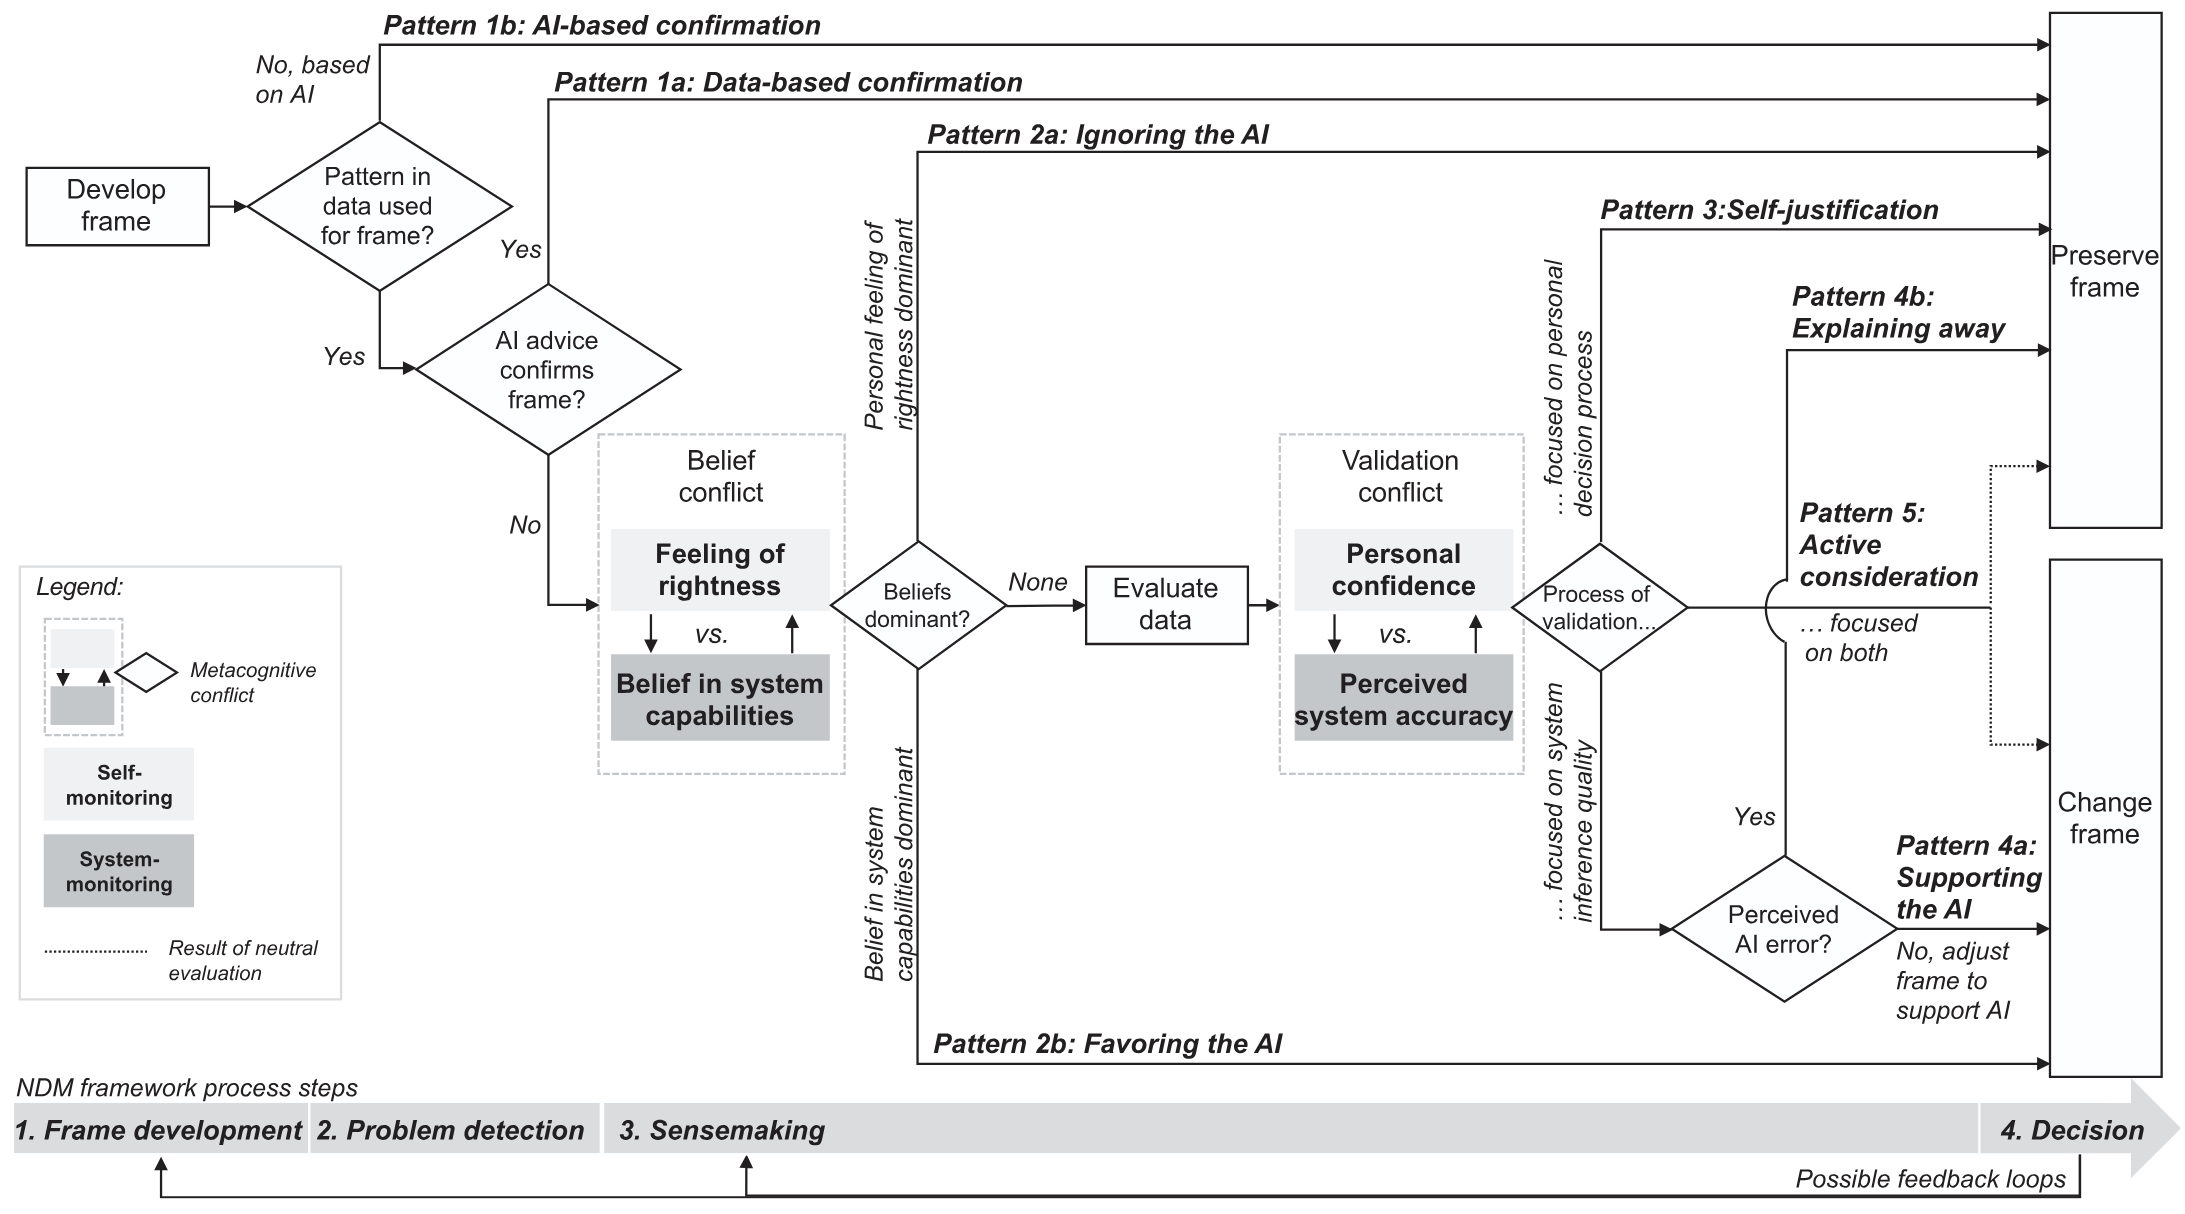
\includegraphics[width=0.8\textwidth]{images/fig-jussupow_model.png}
    \caption[Process Model of AI-Assisted Decision-Making]{Process Model of AI-Assisted Decision-Making \parencite{Jussupow2021}}
    \label{fig:jussupow_process_model}
\end{figure}

In an experiment where researchers performed data analysis tasks with the support of a \ac{LLM}, \textcite{Kazemitabaar2024} found that stepwise task decomposition improves the perceived ease of use of the \ac{AI} and reduced frustration. Users cited improved steering and transparency as key factors for this improvement. Additionally, users reported that the ability to have side conversations with the \ac{LLM} to clarify steps or request additional information was particularly important. Furthermore, users found it easier to verify the output and to intervene and fix errors with stepwise decomposition. These findings suggest, that a \ac{CoT} approach can facilitate an improved perception of transparency and act as an explanation for the \ac{LLM}'s output. This improved perception can facilitate the switch from heuristic to systematic processing when necessary, leading to improved decision-making with \acp{LLM}.

\subsubsection{Psychology of Explanations} \label{sssec:psychology_explanations}

\textcite{Miller2019} reviewed literature from cognitive psychology and social sciences to identify key challenges for \ac{XAI}. A key finding of the review is that explanations can be seen through three different lenses:

\begin{itemize}
    \item Explanations are a \textit{cognitive process}, that involves the selection and organization of information to create an explanation.
    \item The cognitive process results in a \textit{product}, which is the explanation itself.
    \item Explanations are a \textit{social process}, that involves the interaction between the explainer and the explainee.
\end{itemize}

As discussed in Section \ref{sssec:explainability_methods}, much research has been performed into the \textit{cognitive process} (i.e., generation) and the \textit{product} of explanations. However, the \textit{social process} of explanations has been largely neglected in \ac{XAI} research. \textcite{Martens2025} proposed narrative explanations as a way to improve the \textit{social process} of explanations by making them more natural and easier to understand for non-experts. \acp{LLM} offer an additional opportunity to improve the explanation process by enabling interactive explanations through natural language conversations. This allows the \ac{LLM} as the explainer to adapt explanations to the specific needs of the explainee and consequently improve the explanation selection.

Since \textcite{Miller2019} published these findings \textcite{Wachter2017} proposed counterfactual explanations as a way to improve the effectiveness of explanations. Counterfactual explanations align well with the findings of \textcite{Lipton1990}, who identified that humans often do not seek a complete causal explanation, but rather focus on contrasting the event $P$ that occurred with an event $Q$ that did not occur. By focusing on the differences between $P$ (called \textit{fact}) and $Q$ (called \textit{foil}), humans can more easily understand the causal relationships that led to the event. In absence of a clear \textit{foil}, it has to be inferred from context, which emphasizes the importance of explanations being tailored to the explainee.

\subsubsection{AI Anthropomorphism} \label{sssec:ai_anthropomorphism}

Anthropomorphism refers to different facets of the attribution of human characteristics to non-human agents \parencite{Li2022}. In the context of this thesis, the focus lies on the perception of \ac{AI} systems as human-like. This attribution of human-like characteristics can significantly influence how users perceive and therefore interact with the system \parencite{Li2022}. Primarily, anthropomorphism influences users' trust in the system \parencite{Shin2021}. It also influences users acceptance and intention to use the system \parencite{Li2022}. Given these findings, it can be assumed that anthropomorphism acts as a moderating variable, that could reduce users criticality towards \ac{AI} and hinder effective switching from heuristic to systematic processing when necessary.
